% ============================================================
%  Cytron iMD16 Driver Notes + Cheap Campus Delivery Robot Idea
%  First-Year Student Project Proposal -- June 2026
% ============================================================
%  Author:REMAN DEY
%  Advisor: OHfohefhoawuefhoaewhro  ONLYYY MEEEE
% ============================================================

\documentclass[12pt,a4paper]{article}

\usepackage[a4paper, top=1in, bottom=1in, left=1in, right=1in]{geometry}
\usepackage{amsmath}
\usepackage{amssymb}
\usepackage{booktabs}
\usepackage{listings}
\usepackage{xcolor}
\usepackage{hyperref}
\usepackage{titlesec}
\usepackage{parskip}
\usepackage{array}
\usepackage{longtable}
\usepackage{graphicx}
\usepackage{fancyhdr}
\usepackage{enumitem}
\usepackage{caption}
\usepackage{tikz}
\usetikzlibrary{arrows.meta, positioning, shapes.geometric}

\hypersetup{
    colorlinks=true,
    linkcolor=blue!60!black,
    urlcolor=blue!60!black,
    citecolor=blue!60!black,
    pdftitle={Cytron iMD16 Notes and Cheap Campus Delivery Robot},
    pdfauthor={Reman Dey},
}

\definecolor{iitmBlue}{RGB}{18, 18, 18}
\definecolor{iitmGold}{RGB}{198, 15, 51}
\definecolor{codeGray}{RGB}{252, 252, 250}
\definecolor{codeComment}{RGB}{130, 130, 130}
\definecolor{codeKeyword}{RGB}{12, 120, 80}

\titleformat{\section}
  {\color{iitmBlue}\large\bfseries}
  {\thesection}{1em}{}[\color{iitmBlue}\titlerule]

\titleformat{\subsection}
  {\color{iitmBlue!80!black}\normalsize\bfseries}
  {\thesubsection}{1em}{}

\titleformat{\subsubsection}
  {\color{iitmBlue!60!black}\normalsize\itshape\bfseries}
  {\thesubsubsection}{1em}{}

\titlespacing*{\section}{0pt}{18pt}{8pt}
\titlespacing*{\subsection}{0pt}{12pt}{4pt}

\lstdefinestyle{techstyle}{
    backgroundcolor=\color{codeGray},
    commentstyle=\color{codeComment}\itshape,
    keywordstyle=\color{codeKeyword}\bfseries,
    numberstyle=\tiny\color{gray},
    basicstyle=\ttfamily\small,
    breakatwhitespace=false,
    breaklines=true,
    captionpos=b,
    keepspaces=true,
    numbers=left,
    numbersep=5pt,
    showspaces=false,
    showstringspaces=false,
    tabsize=2,
    frame=single,
    rulecolor=\color{iitmBlue!30},
    framesep=4pt,
}
\lstset{style=techstyle}

\pagestyle{fancy}
\fancyhf{}
\fancyhead[L]{\small\textcolor{iitmBlue}{\textbf{iMD16 Notes + Delivery Bot Idea}}}
\fancyhead[R]{\small\textcolor{iitmGold}{\textbf{Reman Dey}}}
\fancyfoot[C]{\small\thepage}
\renewcommand{\headrulewidth}{0.6pt}
\renewcommand{\headrule}{\color{iitmBlue}\hrule width\headwidth height\headrulewidth}

\newcommand{\unitfmt}[1]{\ensuremath{\,\mathrm{#1}}}

\setlength{\headheight}{14.2pt}
\addtolength{\topmargin}{-2.2pt}

\begin{document}

% ============================================================
%  TITLE PAGE
% ============================================================
\begin{titlepage}
    \centering
    \vspace*{1cm}
    {\color{iitmBlue}\rule{\linewidth}{2pt}}\\[0.4cm]
    {\color{iitmBlue}\rule{\linewidth}{0.5pt}}\\[1.2cm]

    {\Huge\bfseries\color{iitmBlue}
        Cytron iMD16 Notes\\[0.3em]
        and a Cheap Campus Delivery Robot Idea
    }\\[0.8cm]

    {\color{iitmGold}\rule{0.6\linewidth}{1pt}}\\[0.6cm]

    {\normalsize
        \textbf{\color{iitmBlue}Reman Dey}\\[0.2em]
        \textbf{\color{iitmBlue}First-Year, Engineering Physics}\\[0.2em]
        \textbf{\color{iitmBlue}Indian Institute of Technology Mandi}\\[0.2em]
    }

    {\color{iitmGold}\rule{0.4\linewidth}{0.5pt}}\\[0.6cm]

    {\large\bfseries June 2026}\\[1.5cm]

    \begin{tabular}{ll}
        \textbf{Document Type:}   & Project Proposal (Club Submission) \\
        \textbf{Hardware Focus:}  & Cytron iMD16 Motor Driver \\[4pt]
        \textbf{Project:}   & Low-Cost Campus Delivery Robot/Campus Cleaner \\[4pt]
        \textbf{Advisor:}         & AeroXMD \\
        \textbf{Campus:}          & IIT Mandi, Himachal Pradesh  \\
    \end{tabular}

    \vfill
    {\color{iitmBlue}\rule{\linewidth}{0.5pt}}\\[0.3cm]
    {\color{iitmBlue}\rule{\linewidth}{2pt}}
\end{titlepage}

% ============================================================
%  TABLE OF CONTENTS
% ============================================================
\newpage
\tableofcontents
\newpage

% ============================================================
%  SECTION 1: INTRO
% ============================================================
\section{Why I'm Writing This}

This is my project proposal for the Robotronics Club. I'm  just a first-year so I don't have a
huge budget or a lot of hands-on experience yet, so I picked something I think I can actually
build this semester.

The report has two parts. First I go through the Cytron iMD16 motor driver in some detail
because that's the one part of the system I'm most confident about and it's the part I had
to actually understand the math for. Second, I sketch out a small delivery-/cleaning robot idea that
uses this driver, but built around parts that are actually affordable for a student club,
not industrial-grade sensors.

I want to be upfront that this is a scaled-down, "let's get something working" proposal,

not a finished engineering design. Things like exact battery sizing, the camera FOV, and
the final BOM will probably change once I start testing.

% ============================================================
%  SECTION 2: MOTOR MATH
% ============================================================
\section{Some Basic Motor Math}

Before picking a driver I wanted to actually understand what a DC motor driver is doing,
not just treat it as a black box, so here's the model I worked through.

\subsection{The Two Equations}

A brushed DC motor is basically an electrical circuit (the coil) connected to a spinning
mechanical part (the shaft + whatever load is on it). You get one equation from circuit
theory and one from rotational mechanics.

\textbf{Electrical side (Kirchhoff's voltage law around the motor coil):}

\begin{equation}
    V(t) = R\,i(t) + L\,\frac{di(t)}{dt} + e_b(t)
    \label{eq:kvl}
\end{equation}

where $V$ is the voltage the driver applies, $R$ is the coil resistance, $L$ is the coil
inductance, $i$ is the current, and $e_b$ is the back-EMF (the voltage the spinning motor
generates on its own, opposing the current).

\textbf{Mechanical side (Newton's second law for rotation):}

\begin{equation}
    T_m(t) = J\,\frac{d\omega(t)}{dt} + B\,\omega(t) + T_L(t)
    \label{eq:newton}
\end{equation}

where $T_m$ is the torque the motor produces, $J$ is the rotational inertia, $\omega$ is
the angular speed, $B$ is friction, and $T_L$ is whatever load torque is fighting the motor
(gravity on a slope, friction, etc).

\subsection{Connecting Them}

Torque and back-EMF are both tied to a single motor constant $K$:

\begin{align}
    T_m(t) &= K \cdot i(t) \\
    e_b(t) &= K \cdot \omega(t)
\end{align}

\subsection{What Happens at Steady State}

If you let the motor settle (no more change in current or speed), the derivative terms
drop out and you can solve for current from Eq.~\eqref{eq:kvl}:

\begin{equation}
    i_{ss} = \frac{V - K\,\omega}{R}
\end{equation}

Plug that into the torque equation and you get the torque--speed line for the motor:

\begin{equation}
    T_m(\omega) = \frac{K}{R}\,V - \frac{K^2}{R}\,\omega
    \label{eq:tm_omega}
\end{equation}

This is the one equation I actually care about, because it tells you the motor's torque
goes down linearly as speed goes up -- which makes sense, since a faster-spinning motor
generates more back-EMF, which fights the current, which lowers torque.

Two useful numbers come out of this:

\begin{equation}
    T_\text{stall} = \frac{K}{R}\,V \quad \text{(torque at zero speed, max current)}
\end{equation}

\begin{equation}
    \omega_0 = \frac{V}{K} \quad \text{(top speed at zero load)}
\end{equation}

\textbf{Why this matters for picking a driver:} the driver basically controls $V$ by
chopping the supply voltage on and off really fast (PWM). Changing the duty cycle shifts
this whole torque-speed line up or down, which is how you get speed control.

% ============================================================
%  SECTION 3: iMD16 EVALUATION
% ============================================================
\section{Cytron iMD16 -- What It Actually Is}



\subsection{Specs (from the datasheet)}

\begin{table}[ht]
\centering
\caption{Cytron iMD16 -- Key Specs}
\label{tab:imd16_specs}
\renewcommand{\arraystretch}{1.3}
\begin{tabular}{@{}lll@{}}
\toprule
\textbf{Parameter} & \textbf{Value} & \textbf{Why it matters} \\
\midrule
Operating voltage      & 7--30\,V DC          & Works with 12\,V or 24\,V batteries \\
Continuous current     & 16\,A per channel    & Plenty for a small wheelchair-size motor \\
Peak current            & 30\,A (under 10\,s)  & Headroom for starting torque / bumps \\
Logic input             & 3--30\,V             & Works directly off a Pi's 3.3\,V GPIO \\
PWM frequency (ext.)    & up to 20\,kHz        & Quiet, doesn't whine \\
Reverse polarity protect & Yes                 & Saves me if I wire the battery backwards \\
Overcurrent/thermal cutoff & Yes               & Won't fry itself if a wheel jams \\
Size                    & $83\times57\times29$\,mm & Small enough to mount easily \\
\bottomrule
\end{tabular}
\end{table}
\begin{figure}
    \centering
    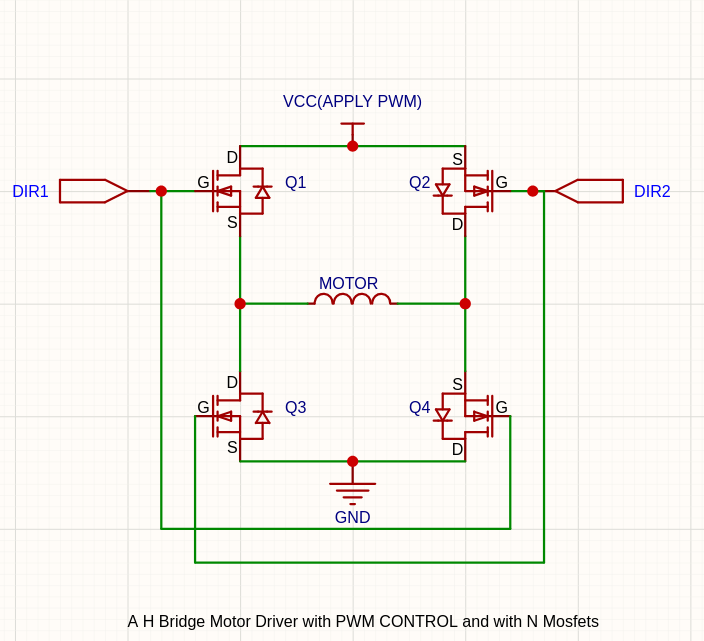
\includegraphics[width=1\linewidth]{Screenshot from 2026-07-01 00-28-14.png}
    \caption{H bridge circuit Diagram made by me}
    \label{fig:sojdfsjf}
\end{figure}

\subsection{Things I Like About It}

\begin{itemize}
    \item \textbf{It's enclosed.} A lot of the cheaper drivers (L298N boards etc.) are
    just bare PCBs. The iMD16 is in a metal case, which seems like a good idea given how
    much it rains here and how dusty the paths get.
    \item \textbf{Logic level is flexible.} It can take anywhere from 3\,V to 30\,V on the
    signal pins, so I don't need any extra level-shifting circuitry between it and a
    Raspberry Pi (which outputs 3.3\,V).
    \item \textbf{Built-in protection.} Reverse polarity and overcurrent protection mean
    I'm less likely to destroy it by wiring something wrong, which, being honest, is a real
    risk for me right now.
\end{itemize}

\subsection{Things to Watch Out For}
\begin{figure}
    \centering
    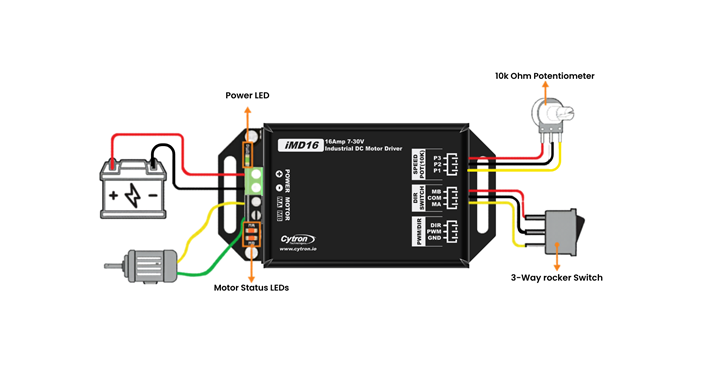
\includegraphics[width=1\linewidth]{abc.png}
    \caption{IMD 16 USAGE}
    \label{fig:placeholder}
\end{figure}
\begin{itemize}
    \item \textbf{No software config.} Everything (braking mode, current limits) is set by
    jumpers/screw terminals, not firmware. So I can't change braking behaviour on the fly
    from code -- I'd have to physically rewire it.
    \item \textbf{No current sensing feedback.} It doesn't tell my code how much current
    it's drawing, so I can't easily detect a stalled wheel in software. I'd need to add an
    external current sensor (like an ACS712 module, which is cheap, around Rs.\,150) if I
    want that later.
    \item \textbf{Braking energy.} If a heavy motor is decelerated suddenly, some energy
    gets pushed back into the supply. With a basic SMPS power supply this could trip an
    overvoltage fault. Running off a battery instead (which I'm planning to do anyway)
    mostly avoids this because batteries can absorb that little kick of energy.
\end{itemize}

\subsection{Is It Overkill or Underpowered for What I Want?}

I did a rough sanity check on the lower and upper ends of what this driver could possibly
be used for, mostly just so I understood the scale of things.

\textbf{Upper end -- could it drive something like an electric bus motor?} No, not even
close. A bus traction motor needs on the order of 150,000\,W. The iMD16 tops out around:

\begin{equation}
    P_\text{max} = 30\,\text{V} \times 16\,\text{A} = 480\,\text{W}
\end{equation}

That's about 300 times too small. Obviously nobody would actually try this, but it helped
me get a feel for where the iMD16 sits.

\textbf{Lower end -- is it overkill for a small campus robot?} Not really. A small
wheelchair-motor-class robot pulling a parcel pannier needs maybe 1--3\,A per motor
under normal driving and a short burst higher than that going up a slope. 16\,A continuous
and 30\,A peak per channel is actually a comfortable margin, not overkill, especially
since I want some safety margin for the steep bits of campus.

\textbf{Conclusion for my project:} the iMD16 is a good fit for a small 12\,V or 24\,V
brushed-motor robot. It would be wrong for anything bigger (e-rickshaw scale and up needs
a completely different, 3-phase BLDC controller).

% ============================================================
%  SECTION 4: OTHER OPTIONS CONSIDERED
% ============================================================
\section{Other Drivers I Looked At}

For completeness, here are a couple of other options I found while researching, in case
the iMD16 turns out to not be available or I need something cheaper/bigger later.

\begin{table}[ht]
\centering
\caption{Other Motor Driver Options}
\label{tab:competitive}
\renewcommand{\arraystretch}{1.3}
\begin{tabular}{@{}lll@{}}
\toprule
\textbf{Driver} & \textbf{Rough Price} & \textbf{Notes} \\
\midrule
Cytron MD20A        & Rs.\,2000  &  Delivers 20A continuously and 60A peak. This model includes convenient manual testing buttons, excellent thermal management (no heatsink required), and works with standard PWM and DIR inputs. \\
BTS7960 module       & Rs.\,300--400  & Higher current (\textasciitilde43\,A claimed) but bare board, no protection \\
Cytron iMD16         & \textasciitilde Rs.\,3{,}200 & What I'm proposing -- enclosed, protected, good logic range \\
Cytron MDDS30        & \textasciitilde Rs.\,5{,}500 & smartdrive, more current, probably overkill for now \\
\bottomrule
\end{tabular}
\end{table}

Honestly the L298N is what most people start with because it's so cheap, but I've read
that it has a pretty bad voltage drop across the H-bridge transistors (no protection
diodes/MOSFETs the way iMD16 has), which wastes power and gets hot. Since the club
already has a couple of iMD16 units sitting around from a previous project, I'm planning
to just reuse one of those rather than buying anything new for this part.

% ============================================================
%  SECTION 5: ROBOT KINEMATICS
% ============================================================
\section{Basic Robot Steering Math (Skid-Steer)}

\subsection{The Idea}

The robot is a simple 4-wheel skid-steer design (think small tank, no steering wheels).
You turn by spinning the left and right wheels at different speeds. It's mechanically
simple -- no servo steering linkage to build.

\begin{figure}[ht]
\centering
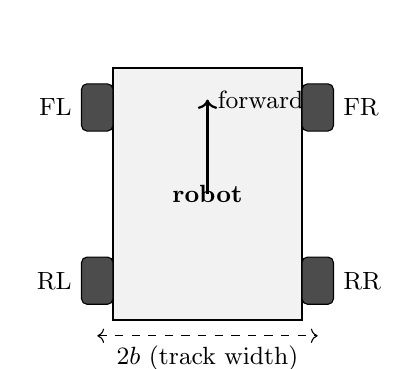
\begin{tikzpicture}[scale=1.0, font=\small]
  \draw[thick, fill=gray!10] (-1.2,-1.6) rectangle (1.2,1.6);
  \node at (0,0) {\textbf{robot}};
  \draw[->, thick] (0,0) -- (0,1.2) node[right]{forward};

  \draw[fill=black!70, rounded corners=2pt] (-1.6,0.8) rectangle (-1.2,1.4);
  \draw[fill=black!70, rounded corners=2pt] (-1.6,-1.4) rectangle (-1.2,-0.8);
  \node[left] at (-1.6, 1.1) {FL};
  \node[left] at (-1.6,-1.1) {RL};

  \draw[fill=black!70, rounded corners=2pt] (1.2,0.8) rectangle (1.6,1.4);
  \draw[fill=black!70, rounded corners=2pt] (1.2,-1.4) rectangle (1.6,-0.8);
  \node[right] at (1.6, 1.1) {FR};
  \node[right] at (1.6,-1.1) {RR};

  \draw[<->, dashed] (-1.4,-1.8) -- (1.4,-1.8) node[midway, below]{$2b$ (track width)};
\end{tikzpicture}
\caption{4-wheel skid-steer layout. Left side wheels and right side wheels each move
together.}
\label{fig:kinematics_geom}
\end{figure}

\subsection{The Equations}

Let $v_L$ and $v_R$ be the left and right side wheel speeds, $b$ be half the track width,
and $r$ the wheel radius. The robot's forward speed $v$ and turn rate $\dot{\psi}$ are:

\begin{equation}
    v = \frac{v_R + v_L}{2}, \qquad \dot{\psi} = \frac{v_R - v_L}{2b}
    \label{eq:fwd}
\end{equation}

And going the other way, if I know what forward speed and turn rate I want, I can solve
for the wheel speeds I need to command:

\begin{equation}
    v_R = v + b\,\dot{\psi}, \qquad v_L = v - b\,\dot{\psi}
    \label{eq:inv}
\end{equation}

Then divide by wheel radius $r$ to get angular speed, and divide by the motor's no-load
speed $\omega_0$ (from Section 2) to get a PWM duty cycle between 0 and 100\%.

\subsection{Quick Numeric Example}

Say $b = 0.25$\,m, $r = 0.075$\,m (small wheel), $\omega_0 \approx 10$\,rad/s. I want to
drive forward at $v = 0.3$\,m/s while turning gently at $\dot{\psi} = 0.2$\,rad/s.

\begin{align*}
    v_R &= 0.3 + 0.25 \times 0.2 = 0.35\,\text{m/s} \\
    v_L &= 0.3 - 0.25 \times 0.2 = 0.25\,\text{m/s}
\end{align*}

Converting to wheel angular speed ($\div r$) and then duty cycle ($\div \omega_0$):

\begin{align*}
    \omega_R &= 0.35/0.075 = 4.67\,\text{rad/s} \rightarrow D_R = 46.7\% \\
    \omega_L &= 0.25/0.075 = 3.33\,\text{rad/s} \rightarrow D_L = 33.3\%
\end{align*}

That's basically the whole control loop -- read a desired speed/turn command, do this
math, send two PWM values to the driver.

% ============================================================
%  SECTION 6: THE ROBOT PROPOSAL
% ============================================================
\section{The Actual Robot Proposal}

\subsection{What I'm Trying to Build}

A small delivery cart that can move along a fixed, pre-mapped route around a part of
campus (not the whole campus -- something more like one hostel block to one
academic block to start) carrying a small parcel. I'm \emph{not} trying to do full
outdoor SLAM or GPS navigation in version 1. That's a lot harder than it sounds, and
honestly outside what I can debug right now as a first-year. Instead I want to use simple
markers (basically big printed QR-code-like tags called ArUco markers) stuck along the
route as landmarks, which is a well-documented beginner-friendly approach.

\subsection{Why I Dropped the Fancy Hardware}

My first draft of this proposal had a Jetson Orin Nano, an OAK-D Pro depth camera, GPS,
and four separate iMD16 drivers -- which added up to almost Rs.\,1.75 lakh. That's not
realistic for a first project, both budget-wise and skill-wise. So I cut it down hard:

\begin{itemize}
    \item \textbf{Jetson Orin Nano $\rightarrow$ Raspberry Pi.} A Pi 4 (or Pi 5 if the
    club already owns one) is more than enough to run OpenCV's ArUco detector and a
    simple control loop. I don't need real-time YOLO segmentation for a slow indoor-ish
    delivery cart on a known path.
    \item \textbf{OAK-D Pro depth camera $\rightarrow$ regular USB webcam.} I just need
    to see ArUco markers and maybe do basic obstacle blob detection, not full depth
    sensing. A normal Rs.\,800 webcam can do this fine for version 1.
    \item \textbf{4$\times$ iMD16} Instead of one driver
    per wheel, I'll wire left-side motors together and right-side motors together (like
    most small skid-steer kits do) and drive them off the two channels of a single iMD16.
    This is a downgrade in flexibility (no independent per-wheel torque vectoring) but
    it's a totally reasonable tradeoff for a v1 robot, and it's the one piece of hardware
    the club already has.
    \item \textbf{GPS module $\rightarrow$ dropped entirely.} Wasn't needed even in the
    original plan since the route is fixed, but now it's extra obviously unnecessary.
\end{itemize}

\subsection{Rough System Sketch}

\begin{lstlisting}[language=bash, caption={What's running on the Pi (rough plan, not final)}]
- webcam_node          : grabs frames from the USB webcam
- aruco_node           : runs OpenCV ArUco detection on each frame
- motor_node           : takes a simple (forward_speed, turn_rate) command
                         and sends PWM + direction to the iMD16
- main_loop            : if marker is visible -> steer toward it
                         if no marker -> go straight slowly, look for one
\end{lstlisting}

I'm planning to write this in plain Python with OpenCV first, not full ROS\,2. ROS\,2 is
genuinely useful but it's a lot of extra infrastructure to learn for a robot this small,
and I think I'll understand my own code better if I write the control loop directly. I
might revisit ROS\,2 in a v2 once I'm more comfortable.

\subsection{Driving the Motors}

Each iMD16 channel takes a PWM signal plus a direction pin. The Pi's GPIO pins run at
3.3\,V logic which is within the iMD16's 3--30\,V input range, so no extra level shifter
is needed.

\begin{lstlisting}[language=Python, caption={Rough motor control sketch}]
def set_motor(pwm_pin, dir_pin, speed):
    # speed is -1.0 to 1.0
    GPIO.output(dir_pin, GPIO.HIGH if speed >= 0 else GPIO.LOW)
    duty = abs(speed) * 100.0
    pwm_pin.ChangeDutyCycle(duty)

def drive(v, omega, b=0.25, r=0.075, w0=10.0):
    # v: forward speed (m/s), omega: turn rate (rad/s)
    v_r = v + b * omega
    v_l = v - b * omega
    speed_r = (v_r / r) / w0
    speed_l = (v_l / r) / w0
    set_motor(PWM_R, DIR_R, speed_r)
    set_motor(PWM_L, DIR_L, speed_l)
\end{lstlisting}

\subsection{Safety}

Since this is a slow, small robot on a known path (not 24\,kg+ moving at speed), I'm not
planning anything fancy here -- just:
\begin{itemize}
    \item A physical kill switch on the battery line I can hit by hand.
    \item Software speed cap so it never drives faster than walking pace.
    \item Basic "stop if marker not seen for N seconds" fallback so it doesn't wander off
    blindly.
\end{itemize}

A proper wireless e-stop system would be a nice v2 addition but it's not something I can
justify spending money on right now.

% ============================================================
%  SECTION 7: BUDGET
% ============================================================
\section{Budget}

This is the part I rewrote the most. Trying to keep the whole thing under Rs.\,30{,}000,
using parts the club either already has or that are easy to get from a local electronics
shop / Amazon / Robu.in.

\subsection{Bill of Materials}

\begin{longtable}{@{}p{4.6cm}rp{3.6cm}rr@{}}
\caption{Budget BOM -- Campus Delivery Robot v1}
\label{tab:bom}\\
\toprule
\textbf{Item} & \textbf{Qty} & \textbf{Notes} & \textbf{Unit (Rs.)} & \textbf{Total (Rs.)} \\
\midrule
\endfirsthead
\multicolumn{5}{c}{\small\itshape (continued)}\\
\toprule
\textbf{Item} & \textbf{Qty} & \textbf{Notes} & \textbf{Unit (Rs.)} & \textbf{Total (Rs.)} \\
\midrule
\endhead
\bottomrule
\endfoot
Cytron iMD16 driver        & 4 & Already owned by the club (Rs.\,0 if reused) & 0 & 0 \\
12\,V DC geared motor (300 RPM) & 4 & Cheap hobby-grade gear motors, left+right pairs wired together & 450 & 1{,}800 \\
Wheels (rubber, 65\,mm)    & 4 & Matched to motor shaft & 120 & 480 \\
12\,V 7\,Ah Lead-Acid battery & 1 & Cheaper than LiFePO$_4$, fine for v1, club may already have a spare & 1{,}400 & 1{,}400 \\
Raspberry Pi 4 (4\,GB)     & 1 & Or reuse one from club inventory if available & 5{,}500 & 5{,}500 \\
MicroSD card (32\,GB)      & 1 & For Pi OS & 400 & 400 \\
USB webcam (720p)          & 1 & For ArUco marker detection & 800 & 800 \\
ArUco markers (printed, laminated) & 15 & Print at campus print shop, laminate at a local shop & 30 & 450 \\
12\,V to 5\,V buck converter & 1 & Powers the Pi off the main battery & 200 & 200 \\
Jumper wires + breadboard  & 1 set & Prototyping & 250 & 250 \\
Toggle switch (kill switch) & 1 & Main power cutoff & 80 & 80 \\
Chassis: plywood/acrylic sheet (cut to size) & 1 & Cheapest option -- can laser-cut at the Fab Lab if free for club projects & 600 & 600 \\
M3 nuts/bolts + standoffs  & 1 set & General assembly & 250 & 250 \\
Cardboard/plastic box for parcel bay & 1 & Reused container, basically free & 100 & 100 \\
Wiring (random gauge, from club stock) & --- & Hopefully scavenged from club leftovers & 300 & 300 \\
\midrule
\multicolumn{4}{r}{\textbf{Subtotal}} & \textbf{12{,}610} \\
\end{longtable}

\subsection{Summary}

\begin{table}[ht]
\centering
\caption{Budget Summary}
\label{tab:bom_summary}
\renewcommand{\arraystretch}{1.3}
\begin{tabular}{@{}lr@{}}
\toprule
\textbf{Item} & \textbf{Cost (Rs.)} \\
\midrule
Subtotal (parts above)        & 12{,}610 \\
Contingency / mistakes buffer (\textasciitilde40\%) & 5{,}040 \\
\midrule
\textbf{Total}                 & \textbf{17{,}650} \\
\bottomrule
\end{tabular}
\end{table}

I put a fairly large 40\% contingency on this because, realistically, I'm going to burn
out a motor driver pin or fry something testing this for the first time, and I'd rather
plan for that honestly than pretend I'll get it right on the first try. Even with that
buffer the total comes to under Rs.\,18{,}000, well inside the Rs.\,30{,}000 target, and
if the Pi and iMD16 are both already available from the club's inventory, the real
out-of-pocket cost could be closer to Rs.\,7{,}000--8{,}000.

\subsection{What I Cut Out (and might add back later)}

\begin{itemize}
    \item \textbf{Depth camera / 3D perception} -- not needed for marker-following on a
    fixed route.
    \item \textbf{GPS/RTK} -- not needed for the same reason, and was never needed even
    in the original full-scale idea.
    \item \textbf{Per-wheel motor drivers} -- one driver with paired channels is enough
    for v1; can revisit if I want real torque vectoring later.
    \item \textbf{LiFePO$_4$ battery} -- a basic lead-acid battery is heavier and less
    efficient but much cheaper and something the club may already have lying around.
    \item \textbf{Wireless e-stop} -- relying on a physical switch for now.
\end{itemize}

% ============================================================
%  SECTION 8: WHY THIS FITS
% ============================================================
\section{Why I Think This Fits the Club}

I know this is a much smaller and less impressive-sounding project than something with a
Jetson and a depth camera, but I think that's actually the point for a first-year
project -- I want to build something I can fully understand and debug myself, on a budget
that doesn't need special approval, using a driver (the iMD16) that the club already has
sitting around. If it works, scaling it up later with a better camera, more drivers, or a
move to ROS\,2 seems like a natural next step instead of something I have to get right on
day one.

% ============================================================
%  SECTION 9: CONCLUSION
% ============================================================
\section{Conclusion}

To sum up what's in this report:

\begin{enumerate}
    \item Worked through the basic DC motor equations (Eqs.~\eqref{eq:kvl}--\eqref{eq:tm_omega})
    to actually understand what the driver is doing instead of treating it as a black box.
    \item Went through the Cytron iMD16 spec sheet and figured out where it fits (good for
    a small 12--24\,V robot, way too small for anything vehicle-scale).
    \item Looked at a couple of cheaper/pricier alternatives for context (L298N, BTS7960,
    MDDS30).
    \item Worked out the skid-steer kinematics (Eqs.~\eqref{eq:fwd}--\eqref{eq:inv}) needed
    to convert a forward-speed/turn-rate command into wheel PWM values.
    \item Put together a stripped-down, budget version of the original delivery-robot idea:
    Raspberry Pi instead of Jetson, a regular webcam instead of a depth camera, one iMD16
    instead of four, and ArUco markers instead of GPS -- bringing the total cost down from
    about Rs.\,1.75\,lakh to under Rs.\,18{,}000.
\end{enumerate}

\vspace{1.5em}
\begin{center}
{\color{iitmBlue}\rule{0.6\linewidth}{1pt}}\\[0.5em]
\textit{Submitted to the Robotronics Club for review -- heppy to get feedback and revise.}\\[0.3em]
{\color{iitmGold}\rule{0.6\linewidth}{0.5pt}}
\end{center}

\end{document}
